\documentclass[12pt]{article}
\setlength{\oddsidemargin}{0in}
\setlength{\evensidemargin}{0in}
\setlength{\textwidth}{6.5in}
\setlength{\parindent}{0in}
\setlength{\parskip}{\baselineskip}


\usepackage[all]{xy}

\usepackage{amsmath,amsfonts,amssymb}
\usepackage{graphicx}
\usepackage{fancyhdr}
\pagestyle{fancy}
\usepackage{hyperref}

\begin{document}

\lhead{{\bf CSCI 3104 \\ Problem Set 9} }
\rhead{Name: \fbox{Keaton Whitehead} \\ ID: \fbox{104668391} \\ {\bf Profs.\ Grochow \& Layer\\ Spring 2019, CU-Boulder}}
\renewcommand{\headrulewidth}{0.5pt}
\phantom{Test}

Quick links \ref{1a} \ref{1b} \ref{1c} \ref{1d} \ref{2} \ref{3}


\vspace{-3mm}
\begin{enumerate}

	\item (30 pts) Bidirectional breadth-first search is a variant of standard BFS for finding a shortest path between two vertices $s,t \in V(G)$. The idea is to run \emph{two} breadth-first searches simultaneously, one starting from $s$ and one starting from $t$, and stop when they ``meet in the middle'' (that is, whenever a vertex is encountered by both searches). ``Simultaneously'' here doesn't assume you have multiple processors at your disposal; it's enough to alternate iterations of the searches: one iteration of the loop for the BFS that started at $s$ and one iteration of the loop for the BFS that started at $t$.
	
	As we'll see, although the worst-case running time of BFS and Bidirectional BFS are asymptotically the same, in practice Bidirectional BFS often performs significantly better.
	
	Throughout this problem, all graphs are unweighted, undirected, simple graphs.
	
	\begin{enumerate}
	\item \label{1a} (5 pts) Give examples to show that, in the worst case, the asymptotic running time of bidirectional BFS is the same as that of ordinary BFS. Note that because we are asking for asymptotic running time, you actually need to provide an infinite family of examples $(G_n, s_n, t_n)$ such that $s_n,t_n \in V(G_n)$, the asymptotic running time of BFS and bidirectional BFS are the same on inputs $(G_n, s_n, t_n)$, and $|V(G_n)| \to \infty$ as $n \to \infty$.
	\\
	\\
	Any line shaped graph family will have the same worst case asymptotic running time for both the bidirectional and the normal BFS. 
	\\
	\\
	Worst case: The S and T starting positions lie at the very end of either side of the line graph.
	\\
	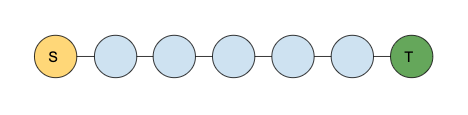
\includegraphics[scale=0.5]{problem1apic1.png}
	\\
	The normal BFS algorithm will have a runtime of O(n) because it will start from one side and travers its way through all the way to the right until it reaches the T vertex. Since S and T are both edge nodes this path will include every node.
	\\
	\\
	\\The Bi-directional BFS algorithm's asymptotic running time would be O(n) because the algorithm will start on either end and work its way to the middle. Again, because they are edge nodes they will include all nodes on the path from S to T because all nodes exist between the two nodes.
	\\
	\\
	\\This is true for the entire line graph family no matter how long the line is, as long as we are always looking at the worst case for both BFS and Bi-directional BFS which involves the starting and ending node at the beginning and the end of the graph. 
	\\
	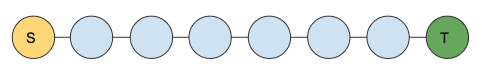
\includegraphics[scale=0.5]{problem1apic2.png}
	\\
	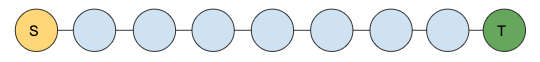
\includegraphics[scale=0.5]{problem1apic3.png}
	\\
	
	\pagebreak
	
	\item \label{1b} (5 pts) Recall that in ordinary BFS we used a \texttt{visited} array (see Lecture Notes 8) to keep track of which nodes had been visited before. In bidirectional BFS we'll need \emph{two} \texttt{visited} arrays, one for the BFS from $s$ and one for the BFS from $t$. Let ``naive bidirectional BFS'' denote an attempted implementation of bidirectional BFS which uses only one {\tt visited} array.  Give an example to show what can go wrong if there's only one \texttt{visited} array. More specifically, give a graph $G$ and two vertices $s,t$ such that some run of a naive bidirectional BFS says there is no path from $s$ to $t$ when in fact there is one.
	\\
	\\
	Before we do anything the visited array in initialized to all no's meaning that none of the nodes have been visited.
	\\
	Let's use this simple example:
	\\
	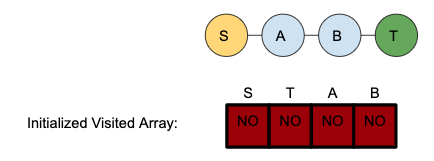
\includegraphics[scale=0.6]{problem1bpic1.png}
	\\
	\\
	When we initiate we will start with node S and mark it visited and its neighbor A. The array now looks like this:
	\\
	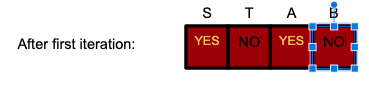
\includegraphics[scale=0.6]{problem1bpic2.png}
	\\
	\\
	In the same iteration we now switch to the T node and mark it visited and its neighbor visited. This is what the array now looks like:
	\\
	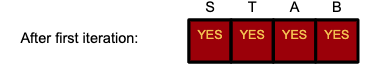
\includegraphics[scale=0.6]{problem1bpic3.png}
	\\
	\\
	This is where our problem occurs because it gets stuck. Since the array is now all marked visited when we look at A or B we will see that all the neighbors are already visited and conclude that this graph is not connected when in fact it is not.
	\pagebreak
	
	\item \label{1c} Consider BFS vs. bidirectional BFS on grids. Namely, let $G_n$ be an $n \times n$ grid, where each vertex is connected to its neighbors in the four cardinal directions (N,S,E,W). Vertices on the boundary of the grid will only have 3 neighbors, and corners will only have 2 neighbors. Let $s_n$ be the midpoint of one edge of the grid, and $t_n$ the midpoint of the opposite edge. For example, for $n=3$ we have:
	
	\[
\xymatrix{
\bullet \ar@{-}[r] \ar@{-}[d] & \bullet \ar@{-}[r] \ar@{-}[d] & \bullet \ar@{-}[d] \\ 
s_3 \ar@{-}[r] \ar@{-}[d] & \bullet \ar@{-}[r] \ar@{-}[d] & t_3 \ar@{-}[d] \\ 
\bullet \ar@{-}[r] & \bullet \ar@{-}[r] & \bullet
}
\]

	\begin{enumerate}
	\item (5 pts) Give an argument as to why BFS starting from $s_n$ searches nearly the entire graph (in fact, a constant fraction of it) before encountering $t_n$. 
	\\
	\\
\begin{minipage}{0.45\textwidth}
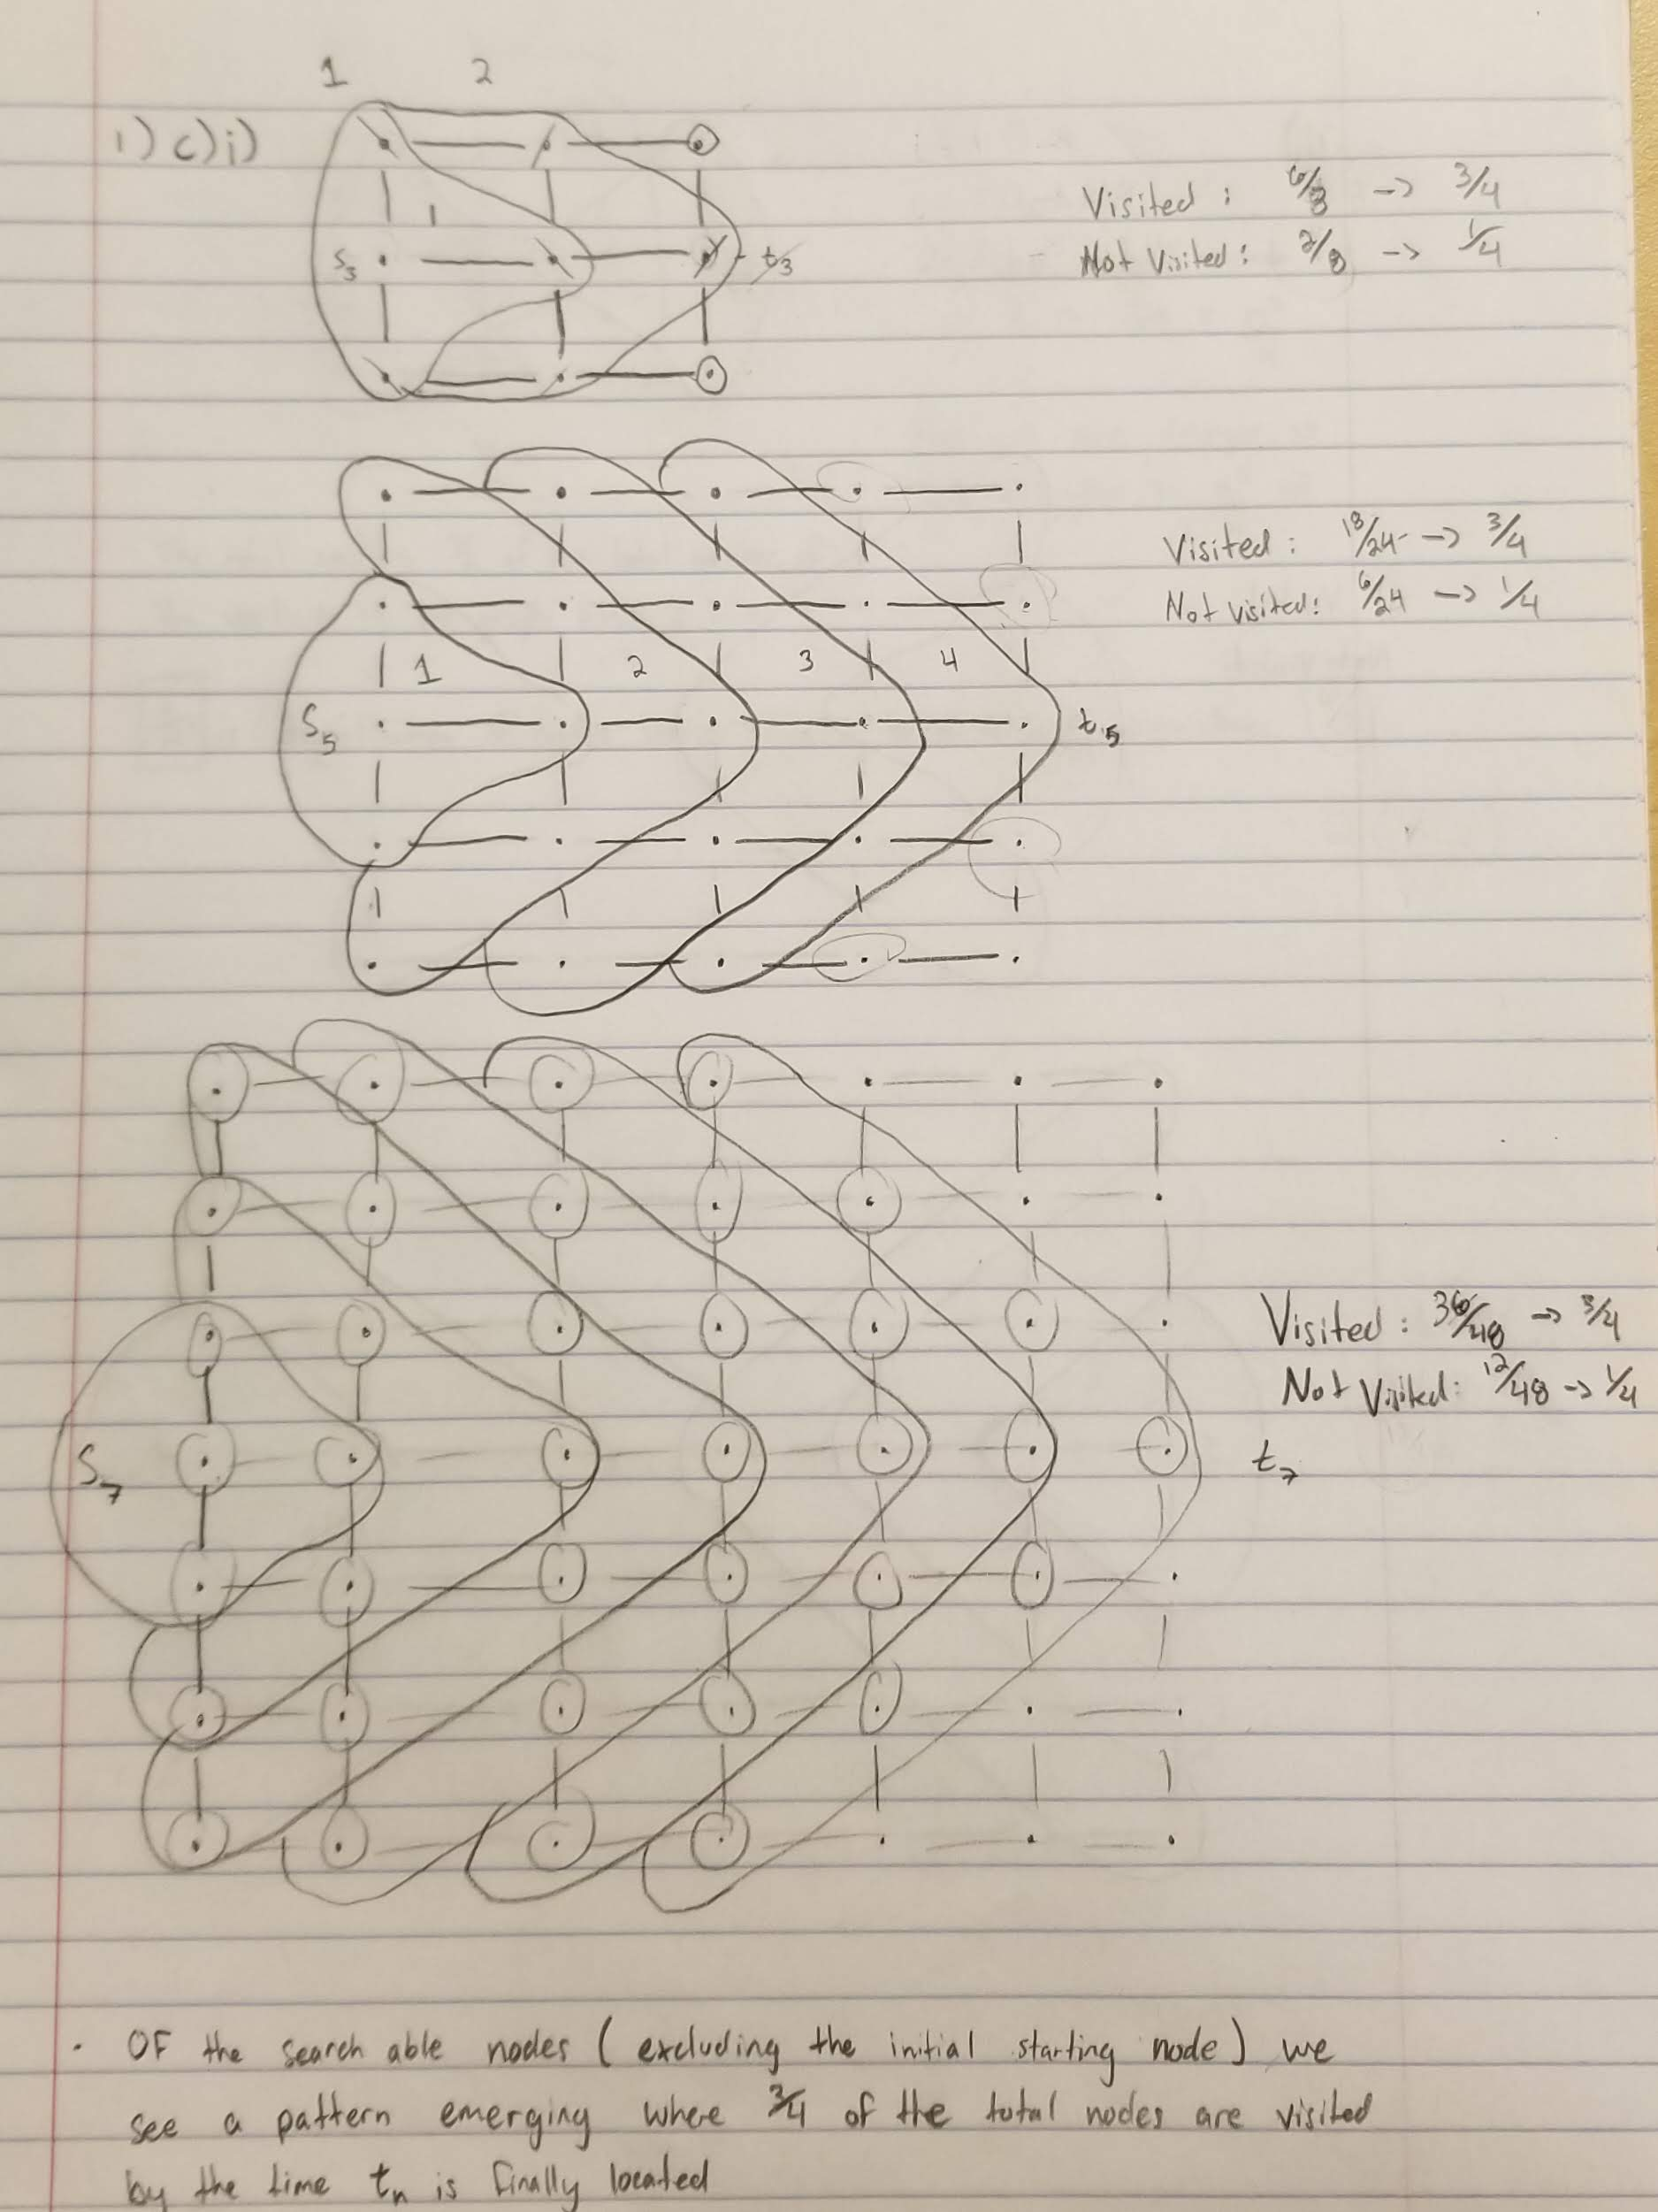
\includegraphics[scale=0.10]{problem1cpic1.png}
\end{minipage}
\begin{minipage}{0.6\textwidth}\raggedright
Of the searchable nodes\\
(excluding the initial starting node)\\
we see a pattern emerging where \\
3/4 of the total nodes are being visited and\\
1/4 are not visited by the time $t_{n}$ is \\
finally reached.\\
This is assuming we do not include the starting \\
node, but if we do, we can see that as n goes to \\
infinity the fractions do approach of 3/4s \\
visited and 1/4 not visited. It is worth noting\\
that if we remove/add the initial node in a \\
graph that is small we it will have a bigger \\
effect on the ratio than if we had a very large \\
graph with a large n.

\end{minipage}
\noindent
\\

	\pagebreak
	
	\item (5 pts) Bidirectional BFS also searches a constant fraction of the entire graph before finding a path from $s_n$ to $t_n$, but a smaller constant fraction than ordinary BFS. Estimate this constant, and give an argument to justify your estimate. Hint: as $n \to \infty$, if you ``zoom out'' the graph starts to look more like the unit square $[0,1] \times [0,1]$ in the real plane $\mathbb{R}^2$. Consider the ``spreading'' picture of BFS / bidirectional BFS and use basic geometric facts.
	\end{enumerate}
	\begin{minipage}{0.45\textwidth}
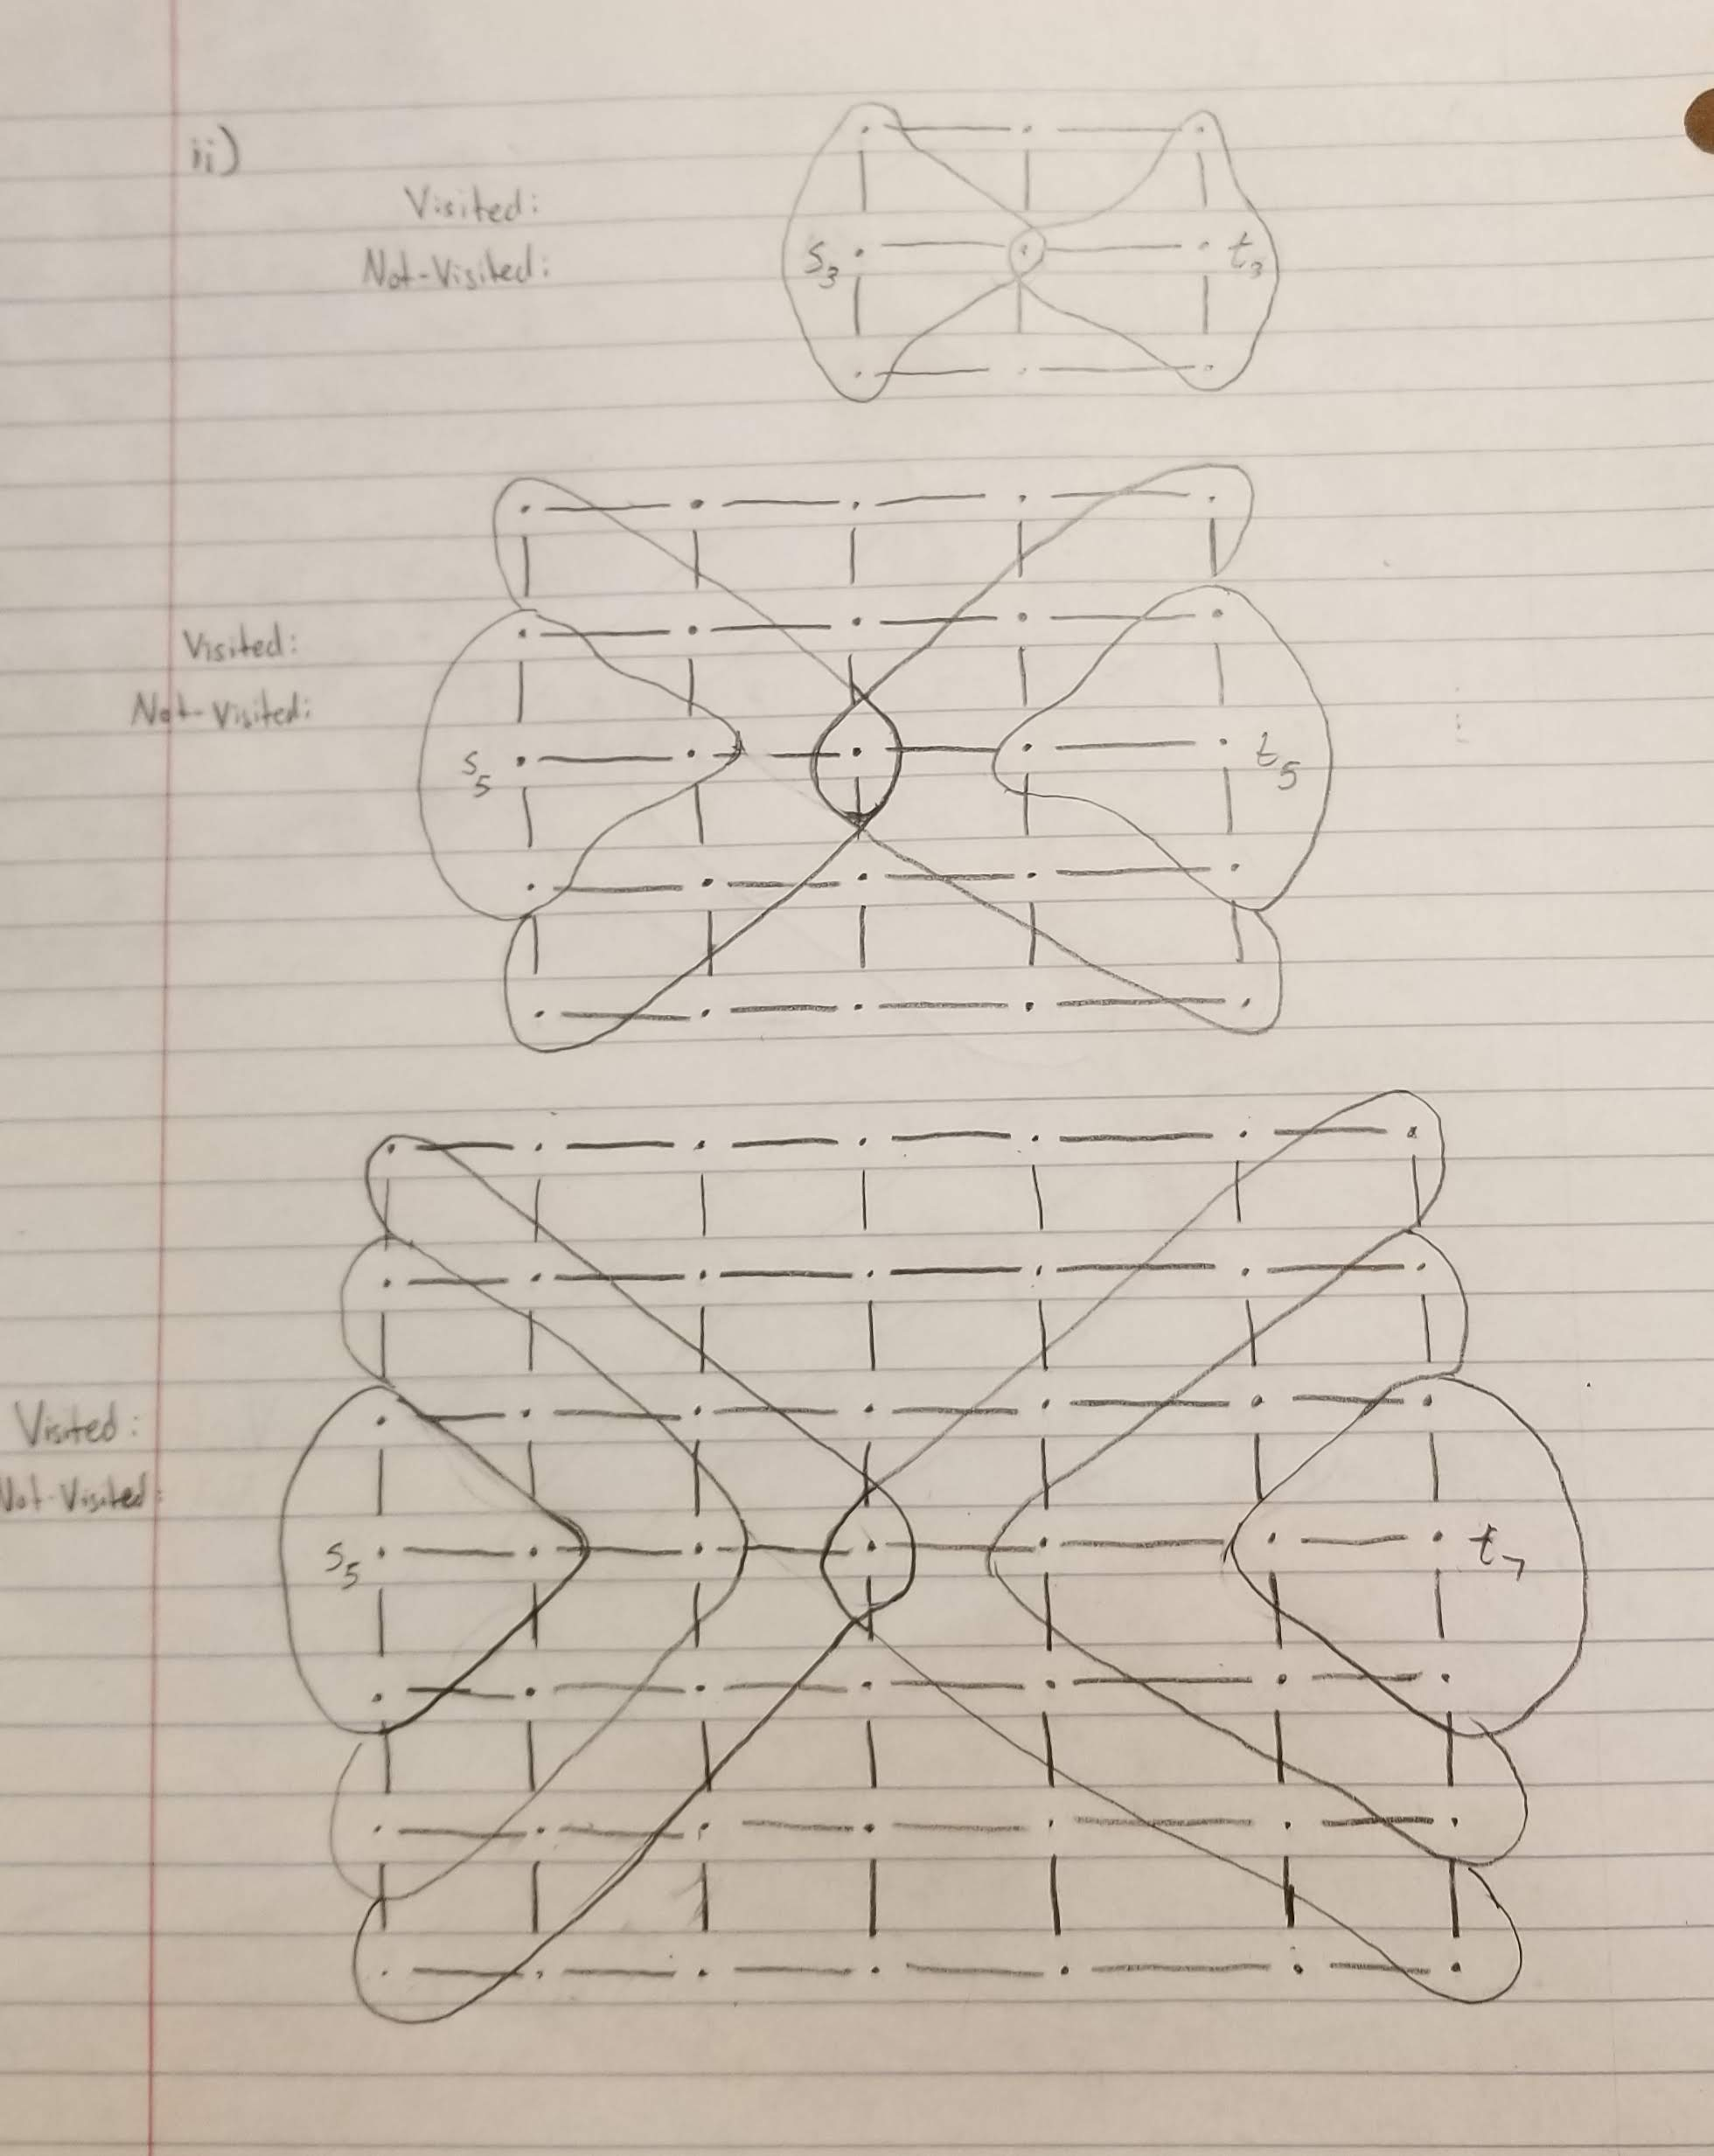
\includegraphics[scale=0.10]{problem1cpic2.png}
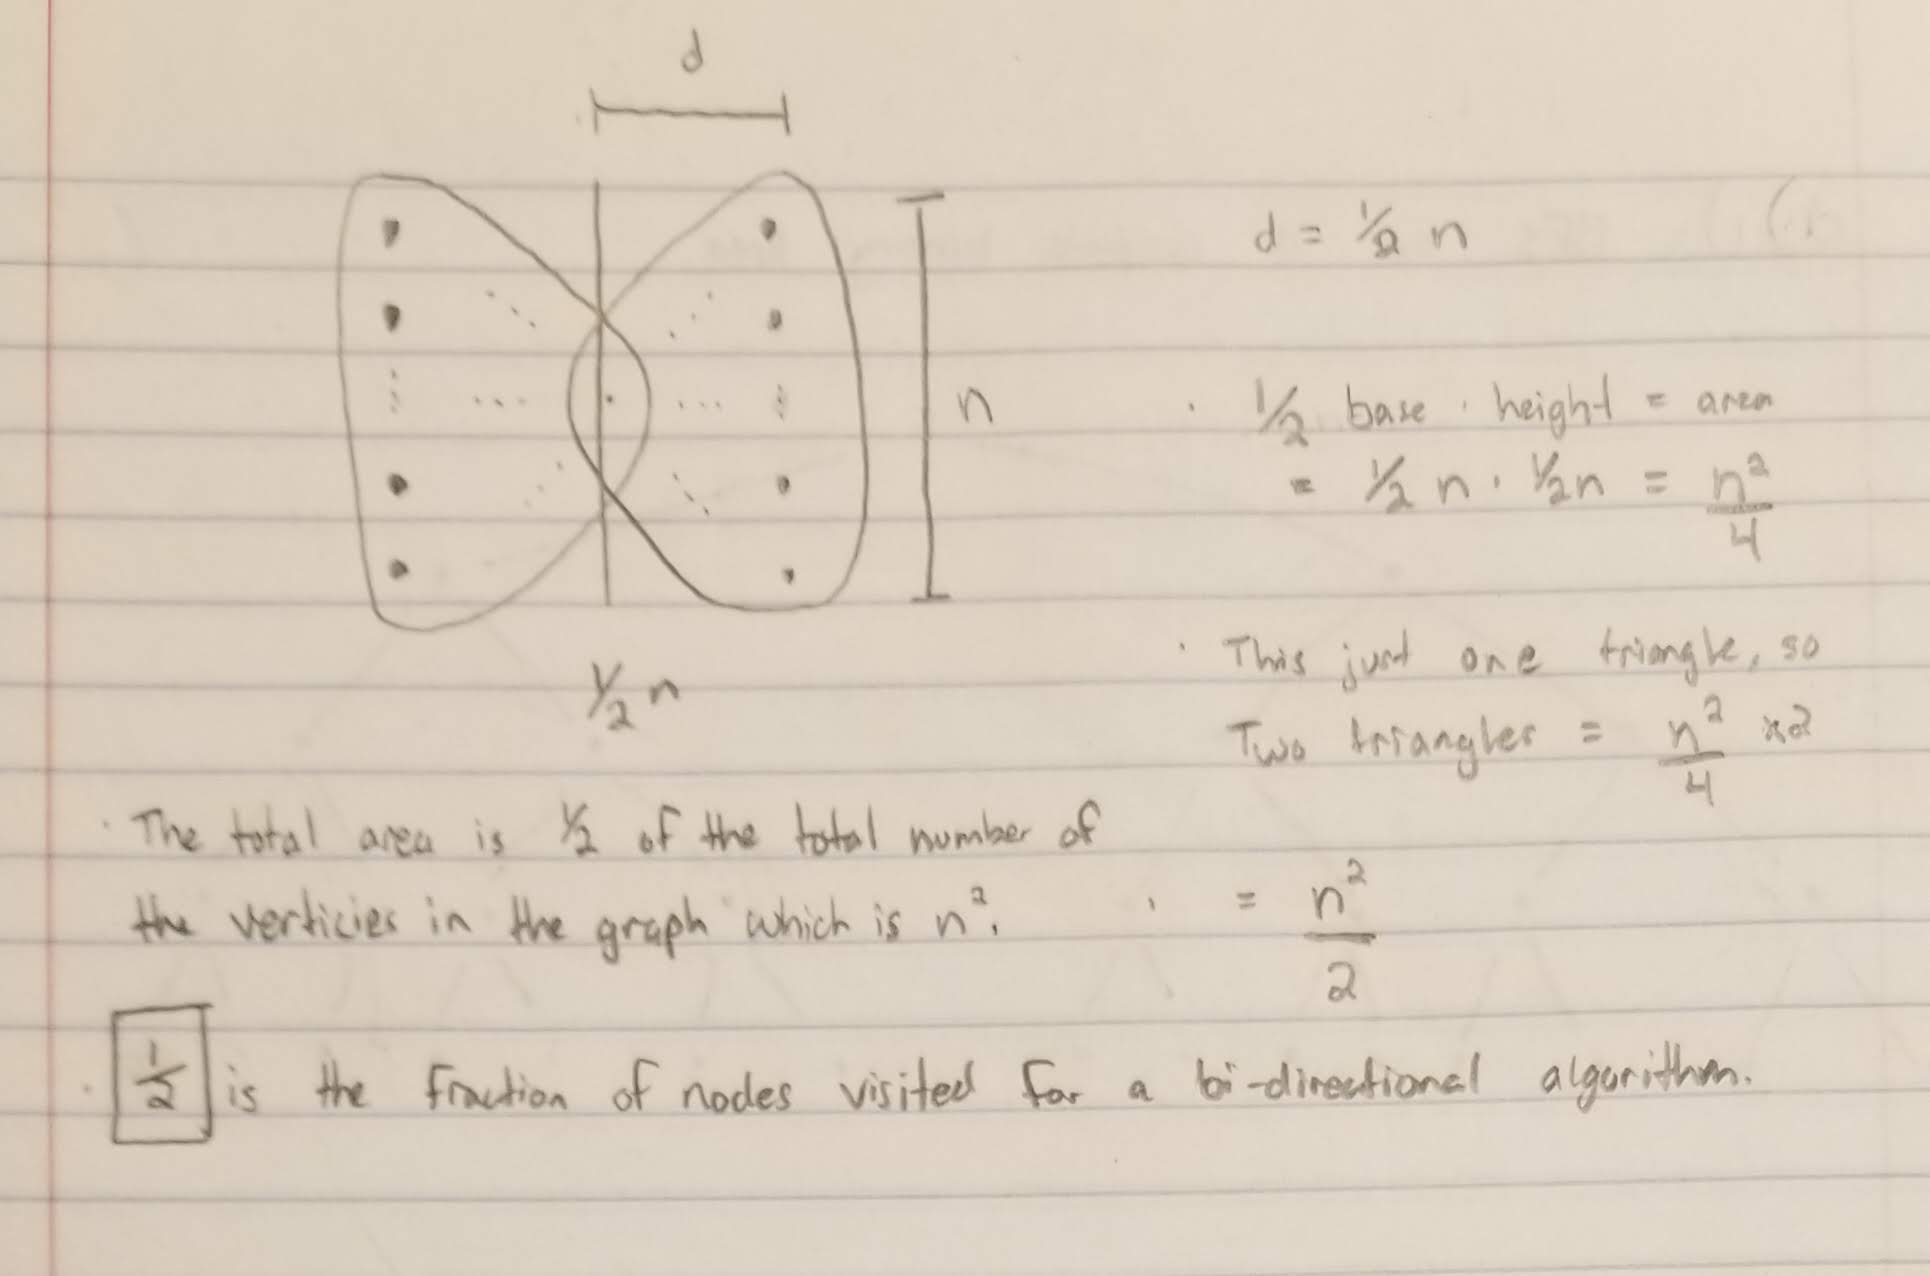
\includegraphics[scale=0.10]{problem1cpic3.png}
\end{minipage}
\begin{minipage}{0.6\textwidth}\raggedright
Using the first picture we can see the pattern \\
that emerges when we scale this problem up to a \\
7-by-7 graph. These are the ratios of each example:\\
\begin{enumerate}
\item Visited: 7/9 = 77.78\\
Not-Visited: 2/9 = 22.22\\
\item Visited: 17/25 = 68.00 \\
Not-Visited: 8/25 = 32.00\\
\item Visited: 31/49 63.27\\
Not-Visited: 18/49 = 36.73 \\
\end{enumerate}
As you can see the more we increase n, the area of \\
the visited nodes decreases as the not-visited\\
nodes' area increases. \\
Now if we look at the second picture we can see that\\
the value it will approach will be 50 percent for \\
both the visited and non-visited areas.\\

\end{minipage}
\noindent
\\


	\pagebreak
	
	\item \label{1d} Consider BFS vs. bidirectional BFS on trees. Let $T_n$ is a complete binary tree of depth $n$. $s_n$ is the root and $t_n$ is any leaf. For example, for $n=3$ we have:
	\[
	\xymatrix{
 	   & & & s_3 \ar@{-}[lld] \ar@{-}[rrd] \\ 
	  & \bullet \ar@{-}[dr] \ar@{-}[dl] & & & & \bullet \ar@{-}[dr] \ar@{-}[dl] \\
	\bullet & & \bullet & & t_3 & & \bullet
	}
	\]
	
	\begin{enumerate}
	\item (5 pts) Prove the asymptotic running time of BFS on $T_n$ starting at $s_n$, where the BFS can stop as soon as it finds a path from $s_n$ to $t_n$.
	\\
	\\
	In class we learned that the complexity of this tree is O(V+E) and in the worst case scenario we have to traverse through all of the nodes and edges. Asymptotically this will be $2^{n} - 1$ + $2^{n} - 2$ which equates to $2^{n}$ so we get a running time of $O(2^{n})$.
	\\
	\\
	Proof:\\
	T(n) = 2T(n-1)+1 \\
	T(n-1) = 2(2T(n-2)+1)+1\\
	....\\
	T(n) = $2^{n} - 1$
	\pagebreak

	\item (5 pts) Prove the asymptotic running time off bidirectional BFS on $T_n$ starting at $(s_n, t_n)$.
	\\
	\\
	This will also result in a asymptotic running time of $O(2^{n})$ as well because $t_n$ will grow up the tree faster than $s_n$ will, but at a constant rate. It will meet at a point that is twice as fast as the BFS because the tree is being traversed both from the top and bottom at the same time while the BFS just traverses down.
	\pagebreak
	
	\end{enumerate}		
	\end{enumerate}
	

	\item \label{2} (10 pts) Let $G=(V,E)$ be a graph with an edge-weight function $w$, and let the tree $T\subseteq E$ be a minimum spanning tree on $G$. Now, suppose that we modify $G$ slightly by decreasing the weight of exactly one of the edges in $(x,y)\in T$ in order to produce a new graph $G'$. Here, you will prove that the original tree $T$ is still a minimum spanning tree for the modified graph $G'$. \\
	 To get started, let $k$ be a positive number and define the weight function $w'$ as
%
\begin{displaymath}
w'(u,v) = \left\{
\begin{array}{ll}
w(u,v) & \textrm{if $(u,v)\not= (x,y)$} \\
w(x,y)-k & \textrm{if $(u,v)=(x,y)$} \enspace .
\end{array}\right.
\end{displaymath}
%
Now, prove that the tree $T$ is a minimum spanning tree for $G'$, whose edge weights are given by $w'$.
	\\
	\\
	We know that the graph T is a minimum spanning subtree of G = (V,E). What makes T a valid :
\begin{enumerate}
\item It is non-cyclical 
\item Has $|E|-1$ edges
\item Contains all the vertices of G
\end{enumerate}
This satisfies all of the requirements because when you reduce the weight of an edge by one it does not create a cycle, it does not remove an edge, and it does not remove any vertices so it is still a minimum spanning tree.
		\pagebreak





	\item \label{3} (20 pts) Professor Snape gives you the following unweighted graph and asks you to construct a weight function $w$ on the edges, using positive integer weights only, such that the following conditions are true regarding minimum spanning trees and single-source shortest path trees:
	\begin{itemize}
	\itemsep-0.1pt
	\item The MST is distinct from any of the seven SSSP trees.
	\item The order in which Jarn\'ik/Prim's algorithm adds the safe edges is different from the order in which Kruskal's algorithm adds them.
	\item Bor$\rm{\dot{u}}$vka's algorithm takes at least two rounds to construct the MST.
	\end{itemize}
	Justify your solution by (i) giving the edges weights, (ii) showing the corresponding MST and all the SSSP trees, and (iii) giving the order in which edges are added by each of the three algorithms. (For Bor$\rm{\dot{u}}$vka's algorithm, be sure to denote which edges are added simultaneously in a single round.)

% ----- FIGURE 1 : adjacency_list.eps -----
\begin{figure}[h!]
\begin{center}
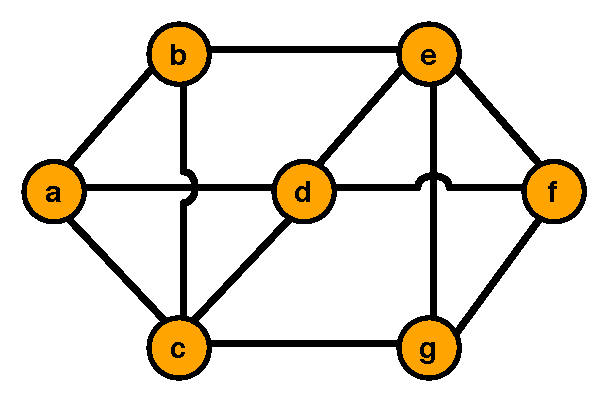
\includegraphics[scale=0.7]{graph_mst.pdf} 
\end{center}
\end{figure}
% ----------
These are all of the SSSP Trees + (i,ii)\\
The order for the SSSP Trees all start at the specified node noted next to each graph.\\

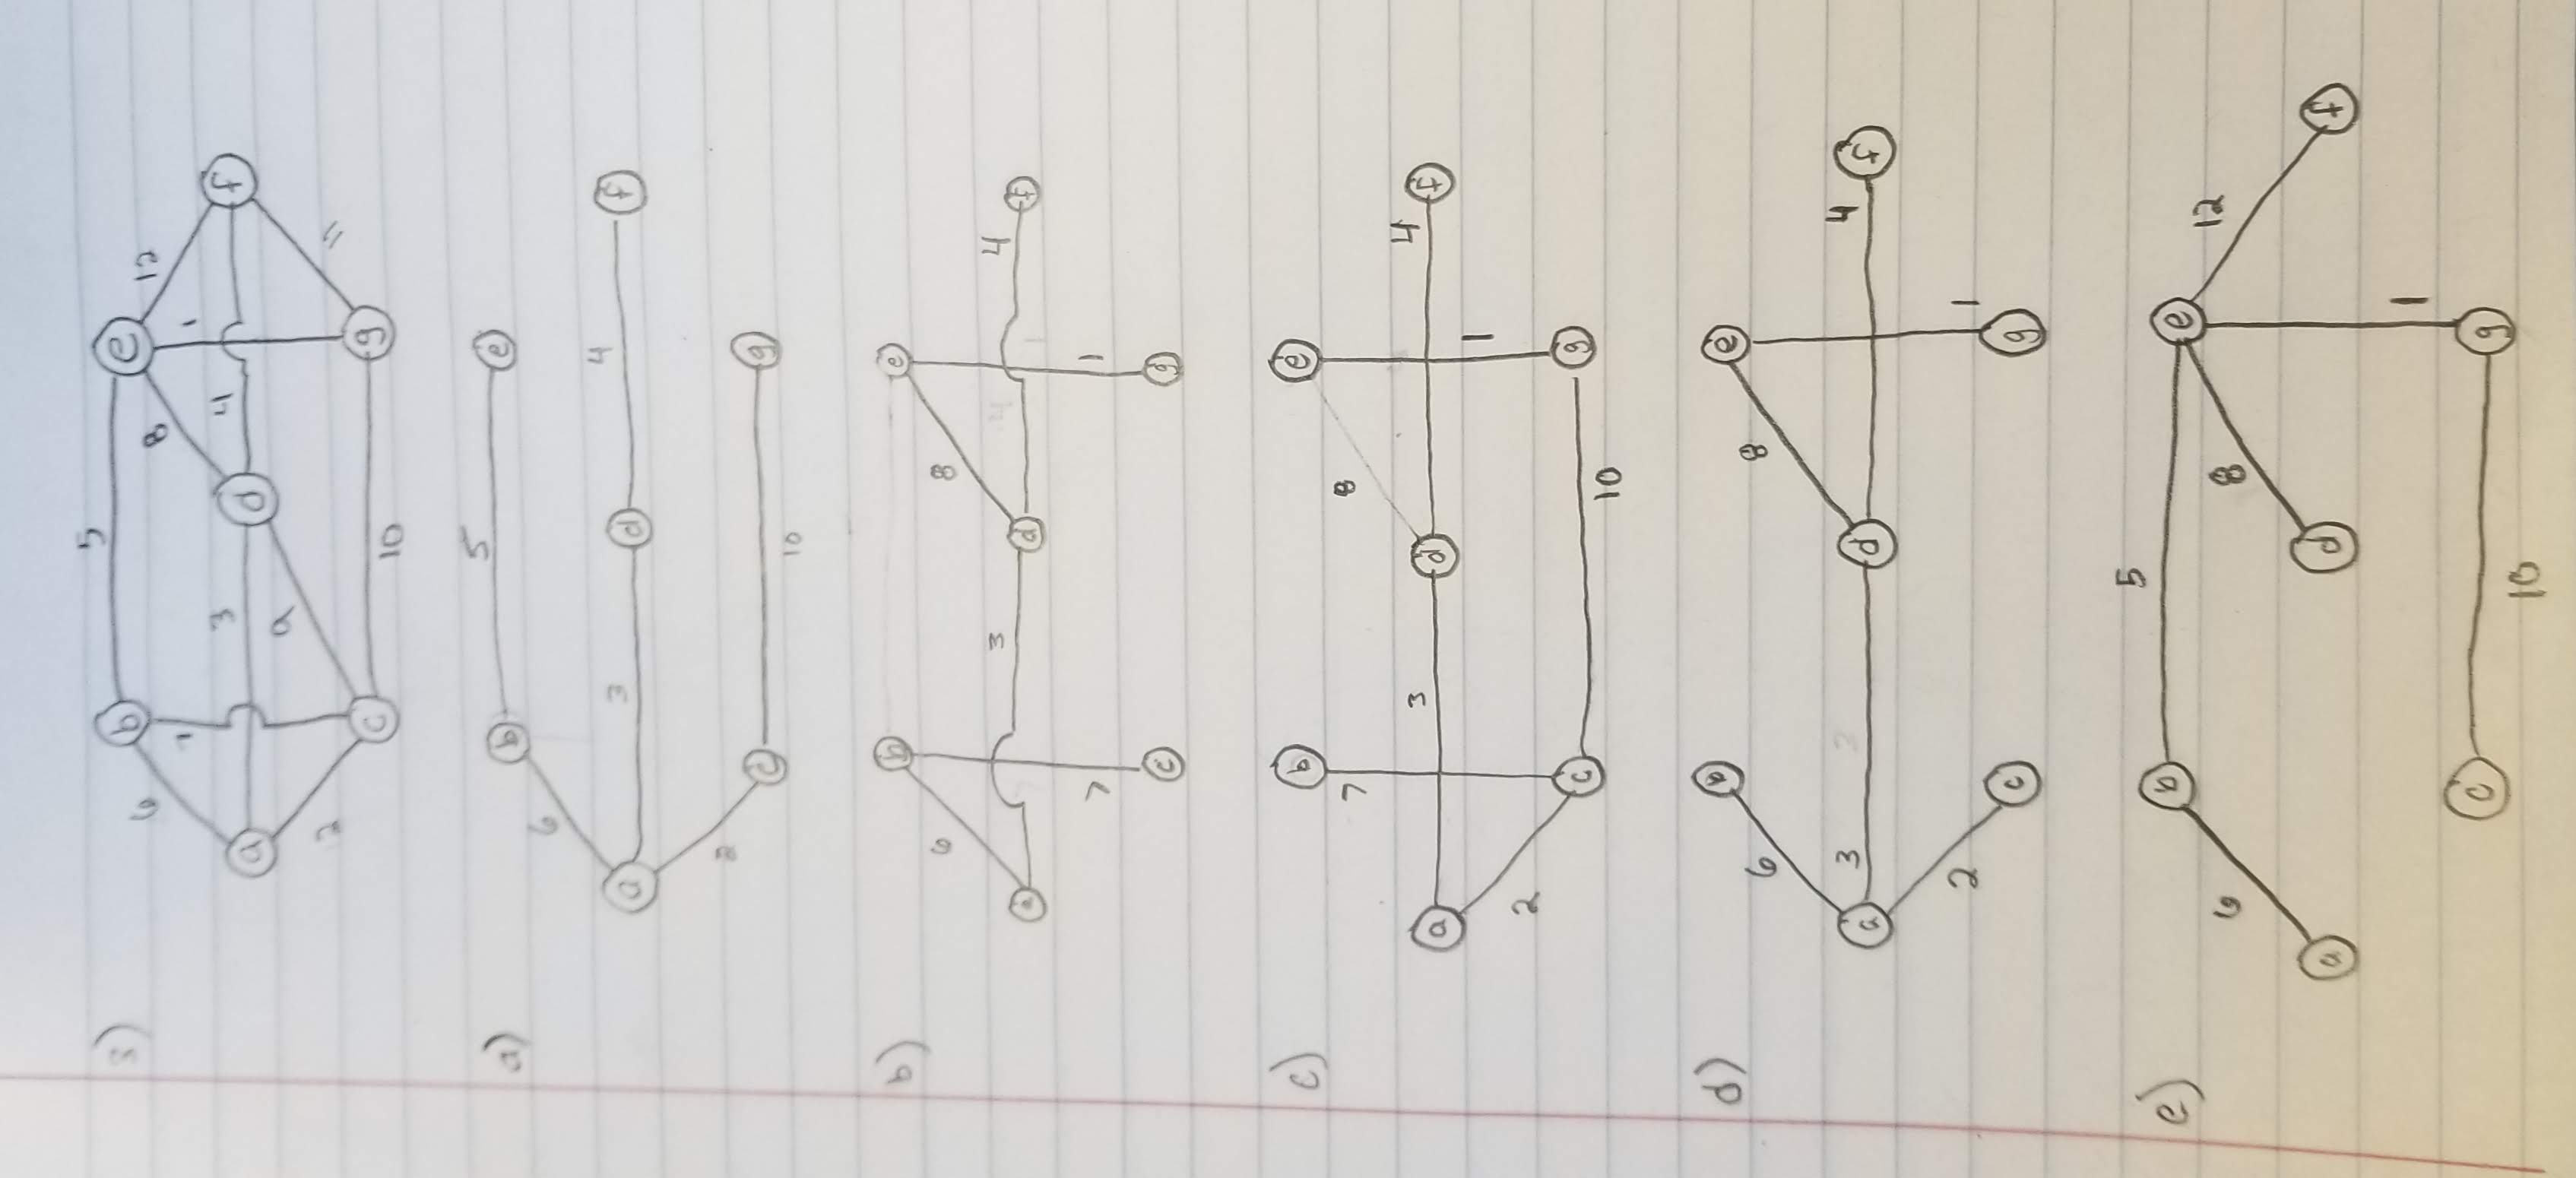
\includegraphics[scale=0.08]{problem3pic1.png}
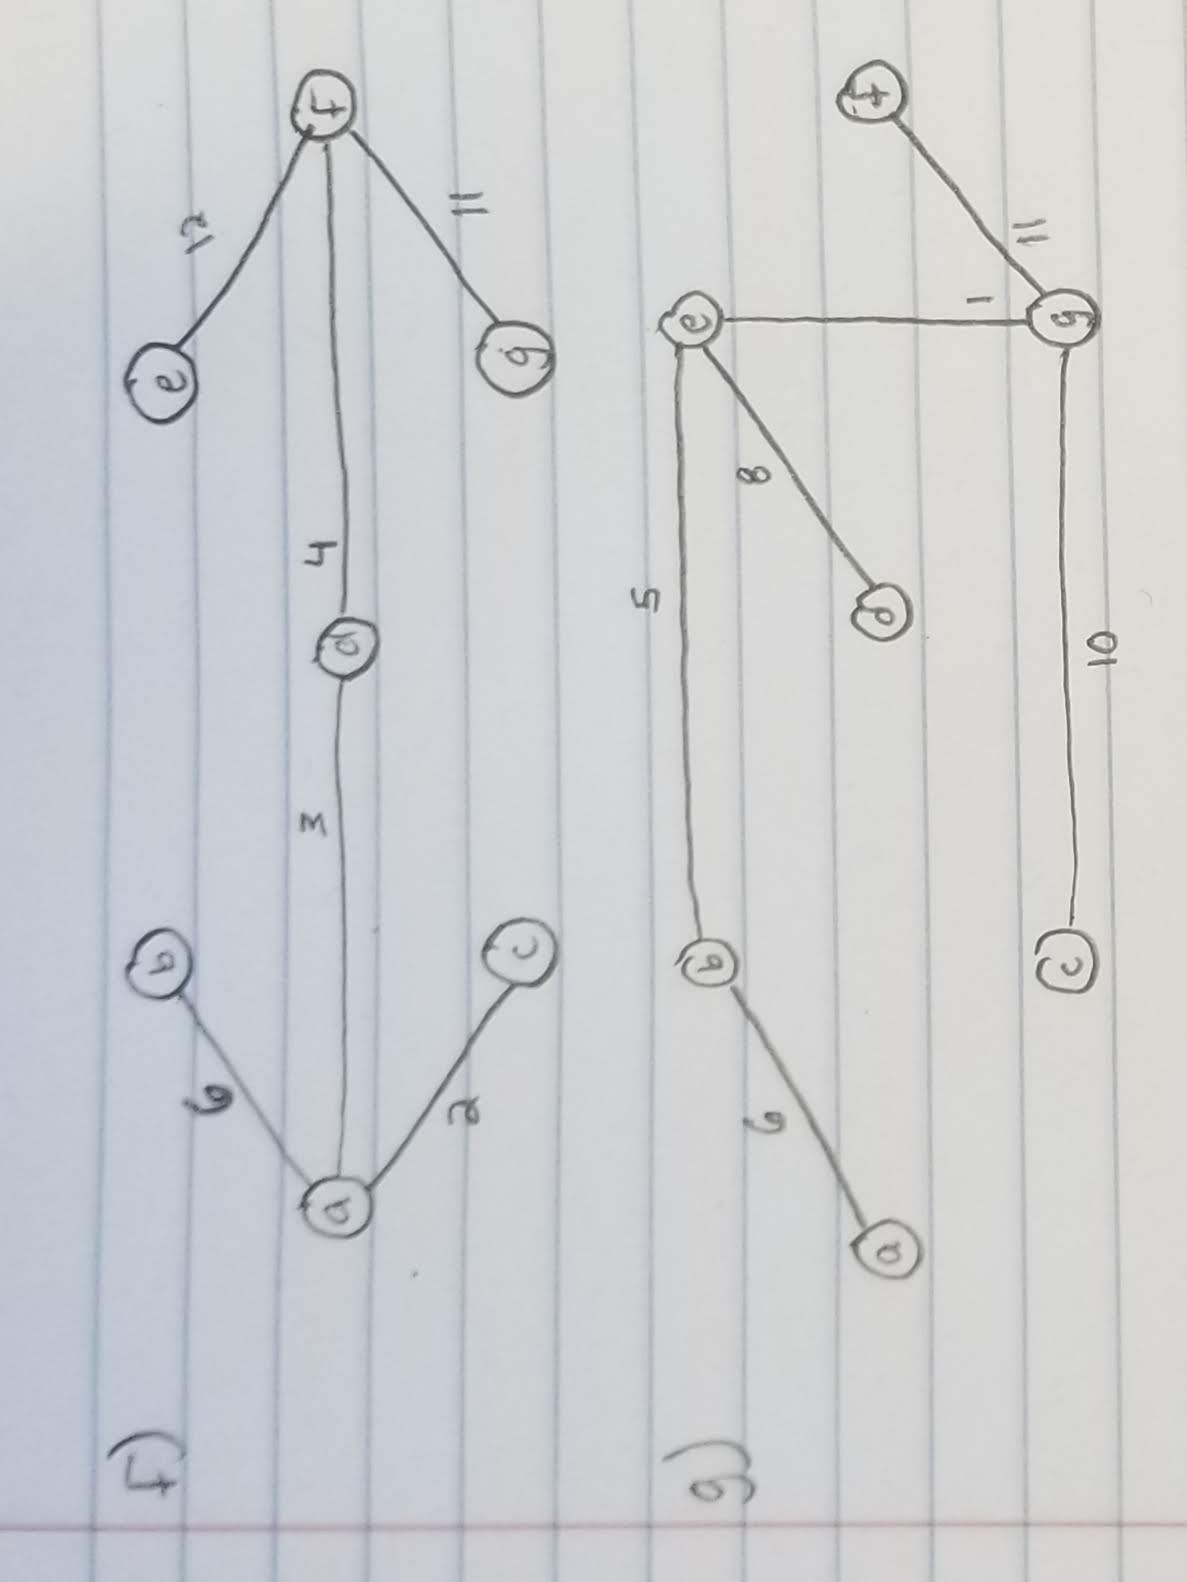
\includegraphics[scale=0.08]{problem3pic2.png}
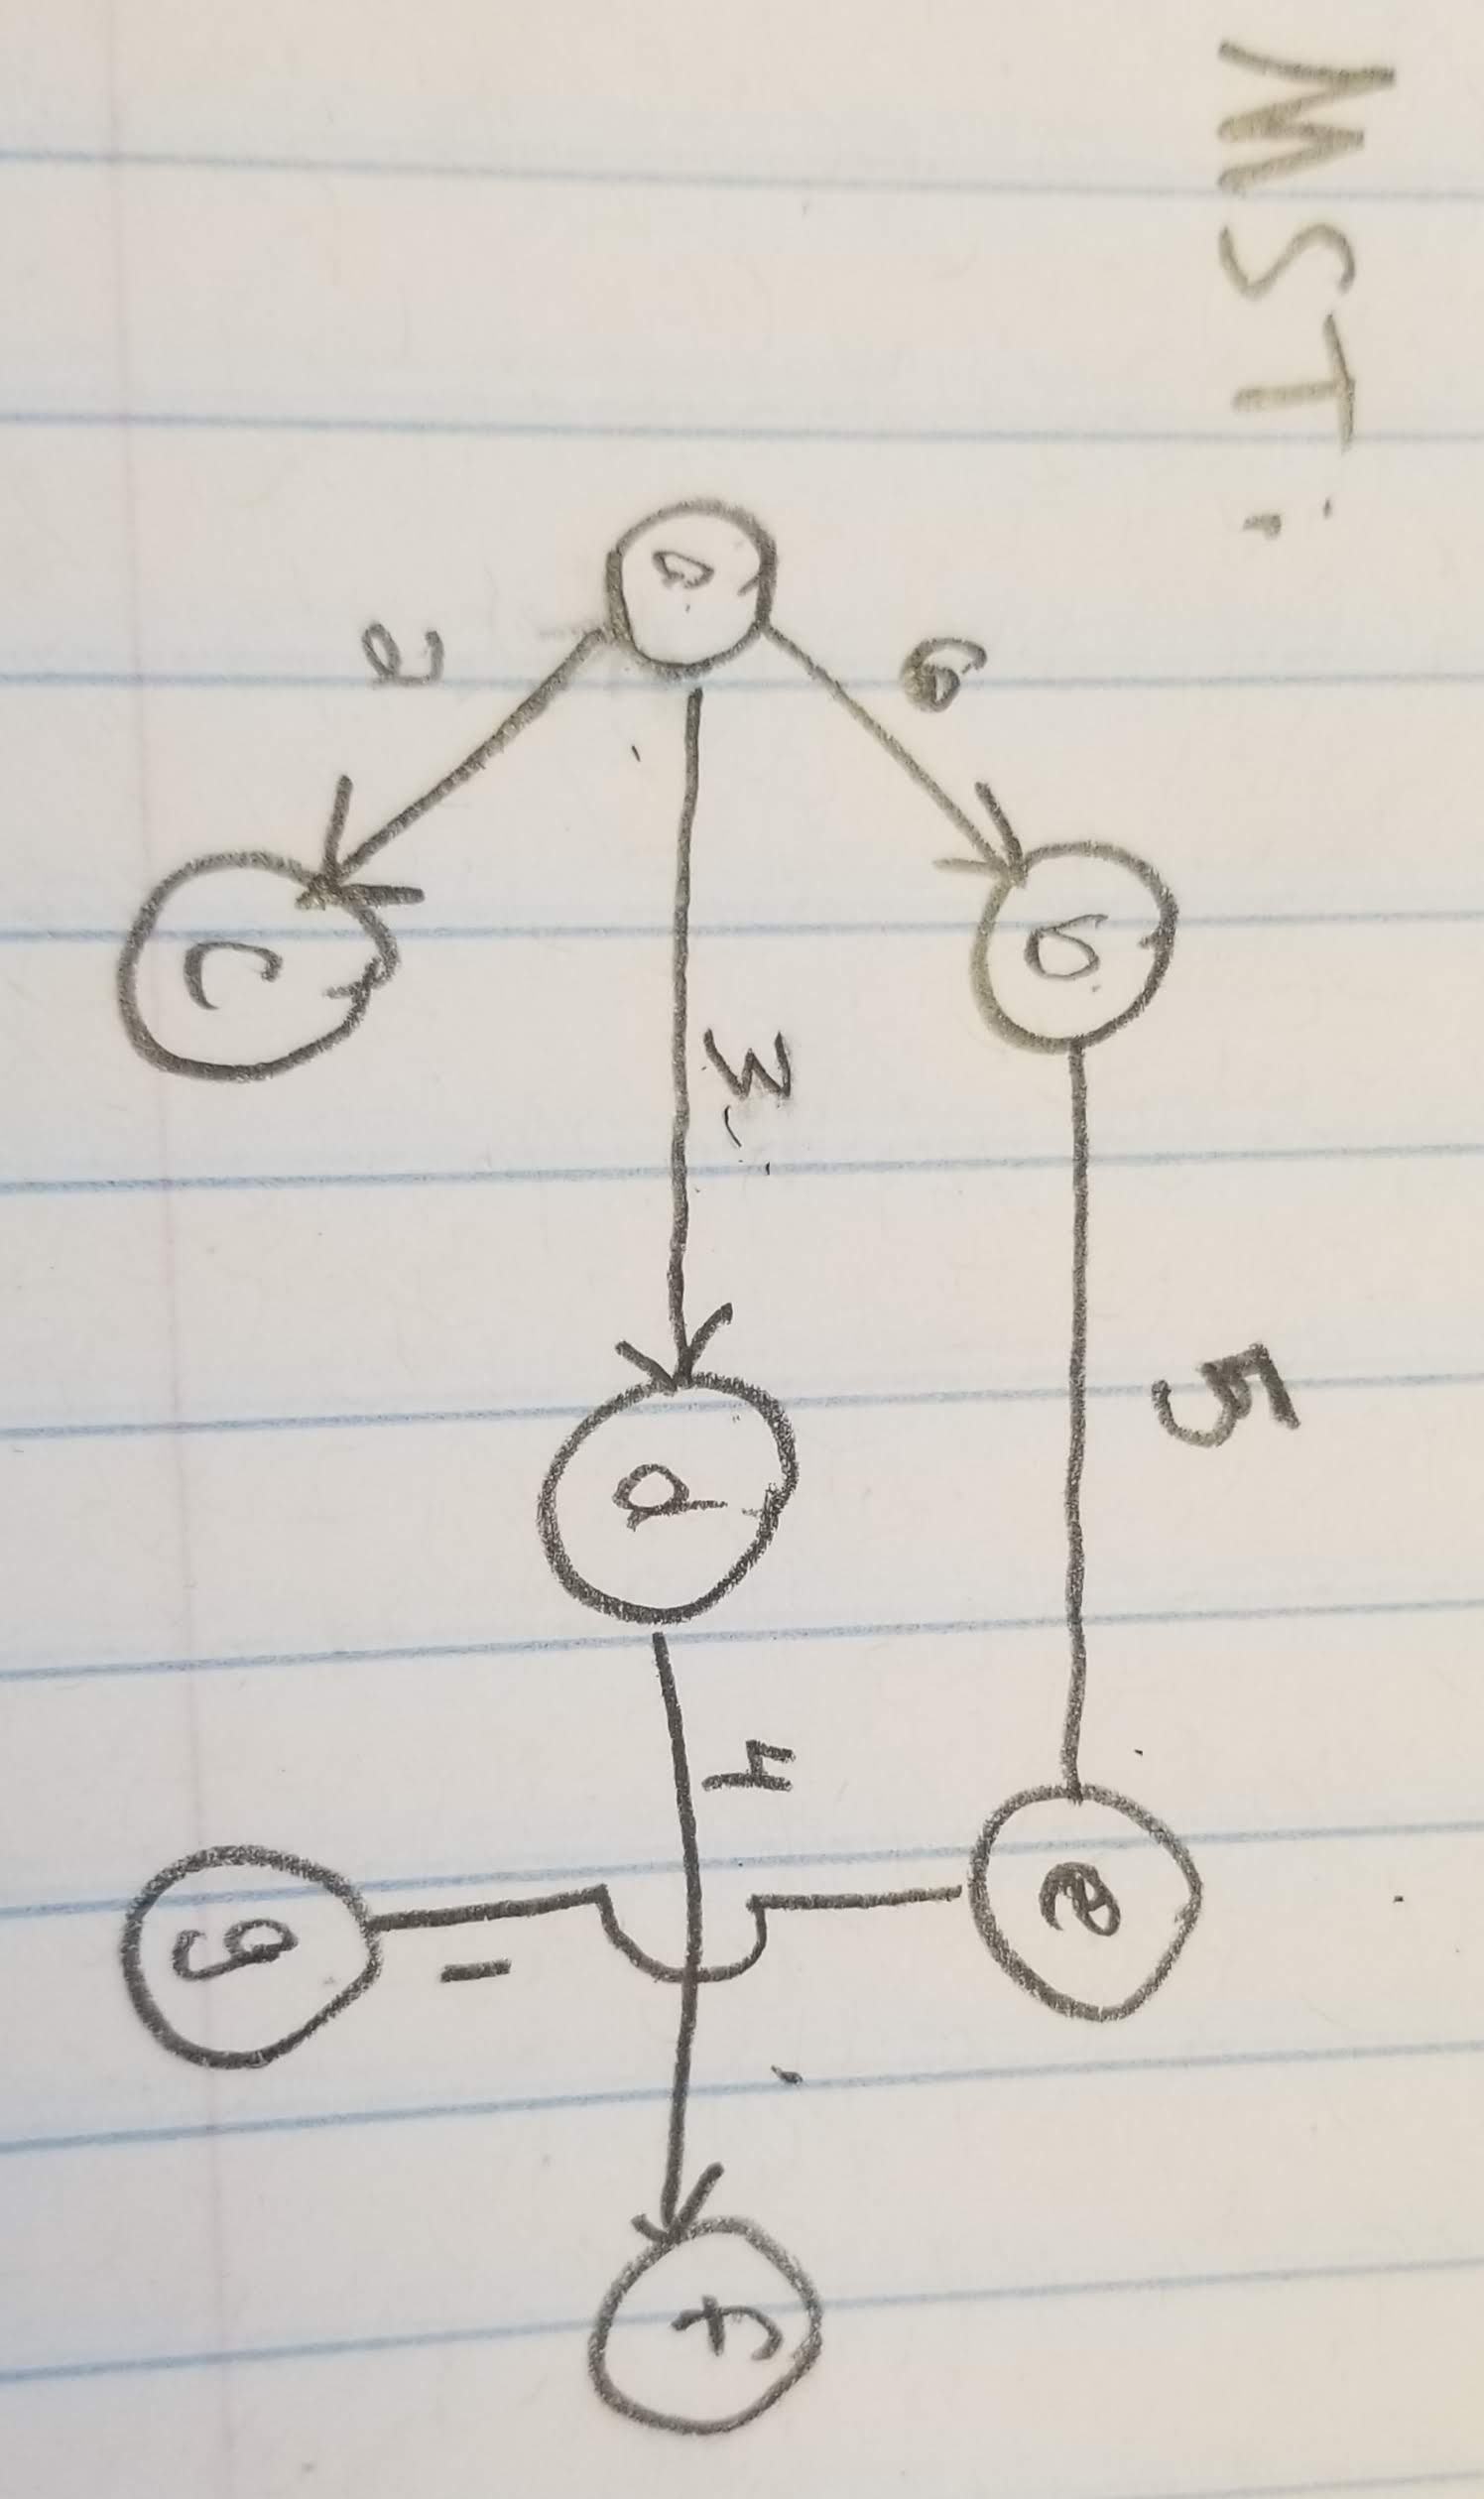
\includegraphics[scale=0.05]{problem3pic3.png}
\pagebreak
\\
Here is how Prim's algorithm adds the safe edges:\\
\\
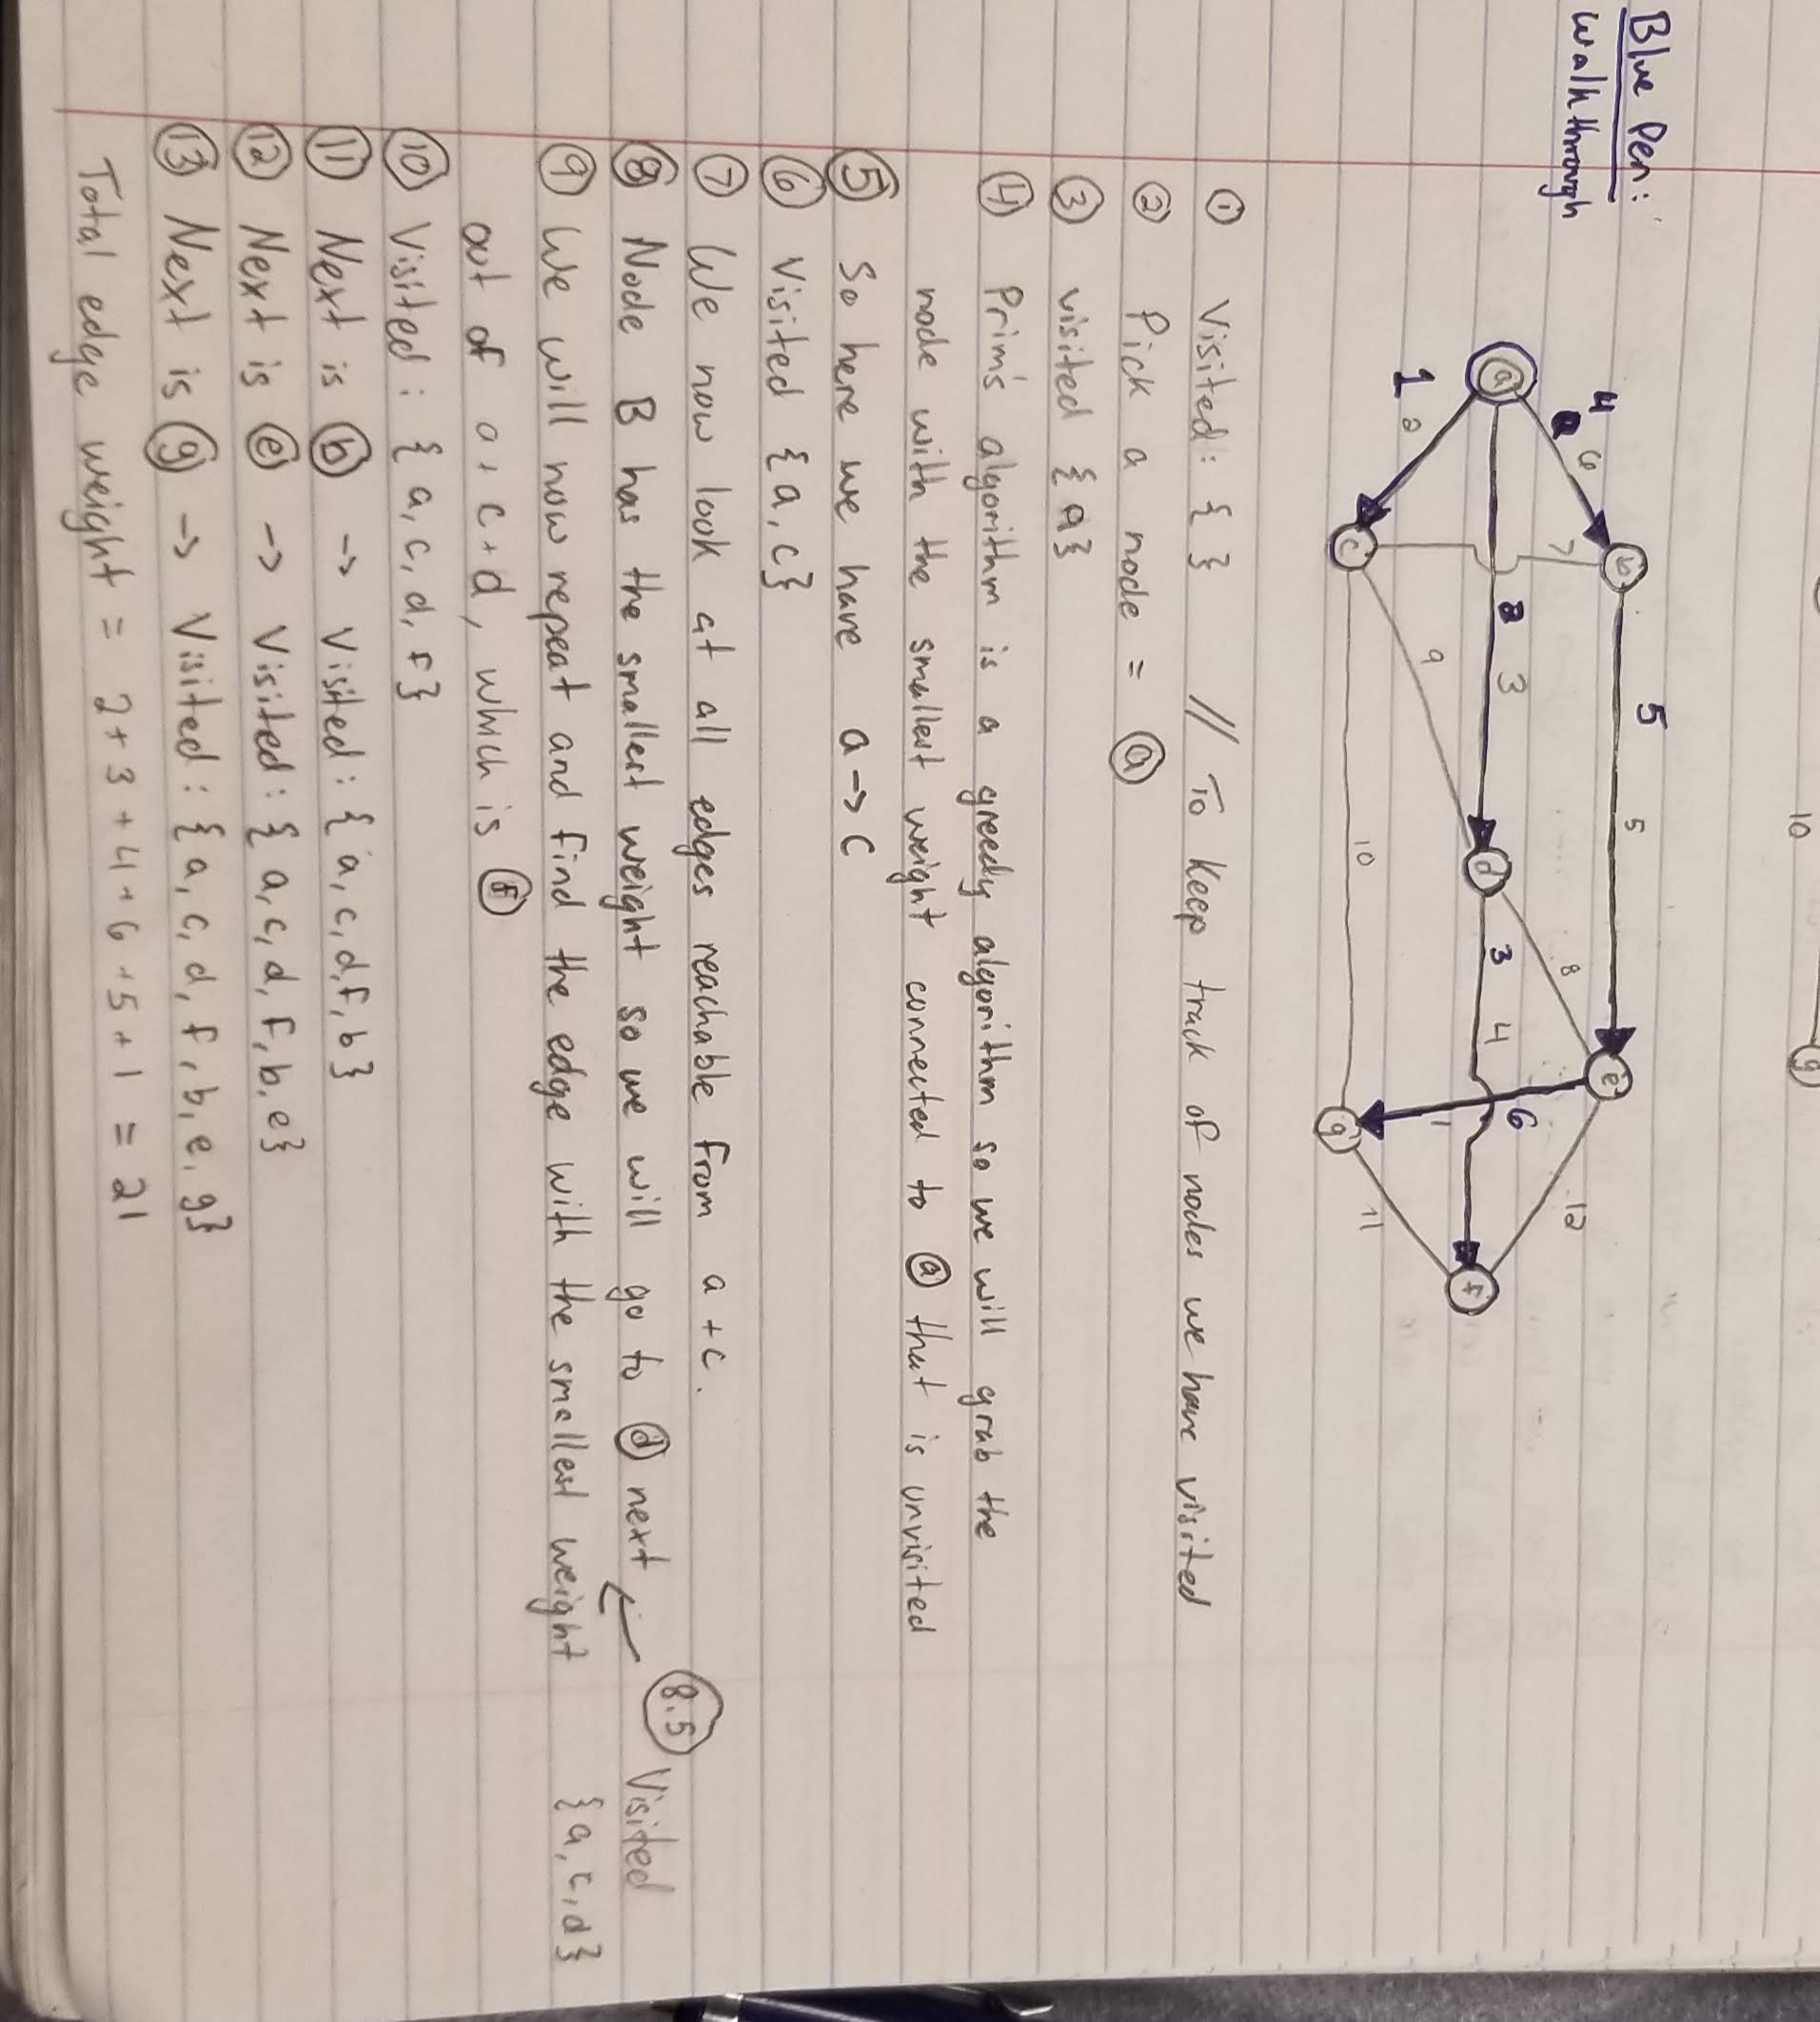
\includegraphics[scale=0.10, angle =90]{problem3pic4.png}\\
Here is Kruskal's algorithm\\
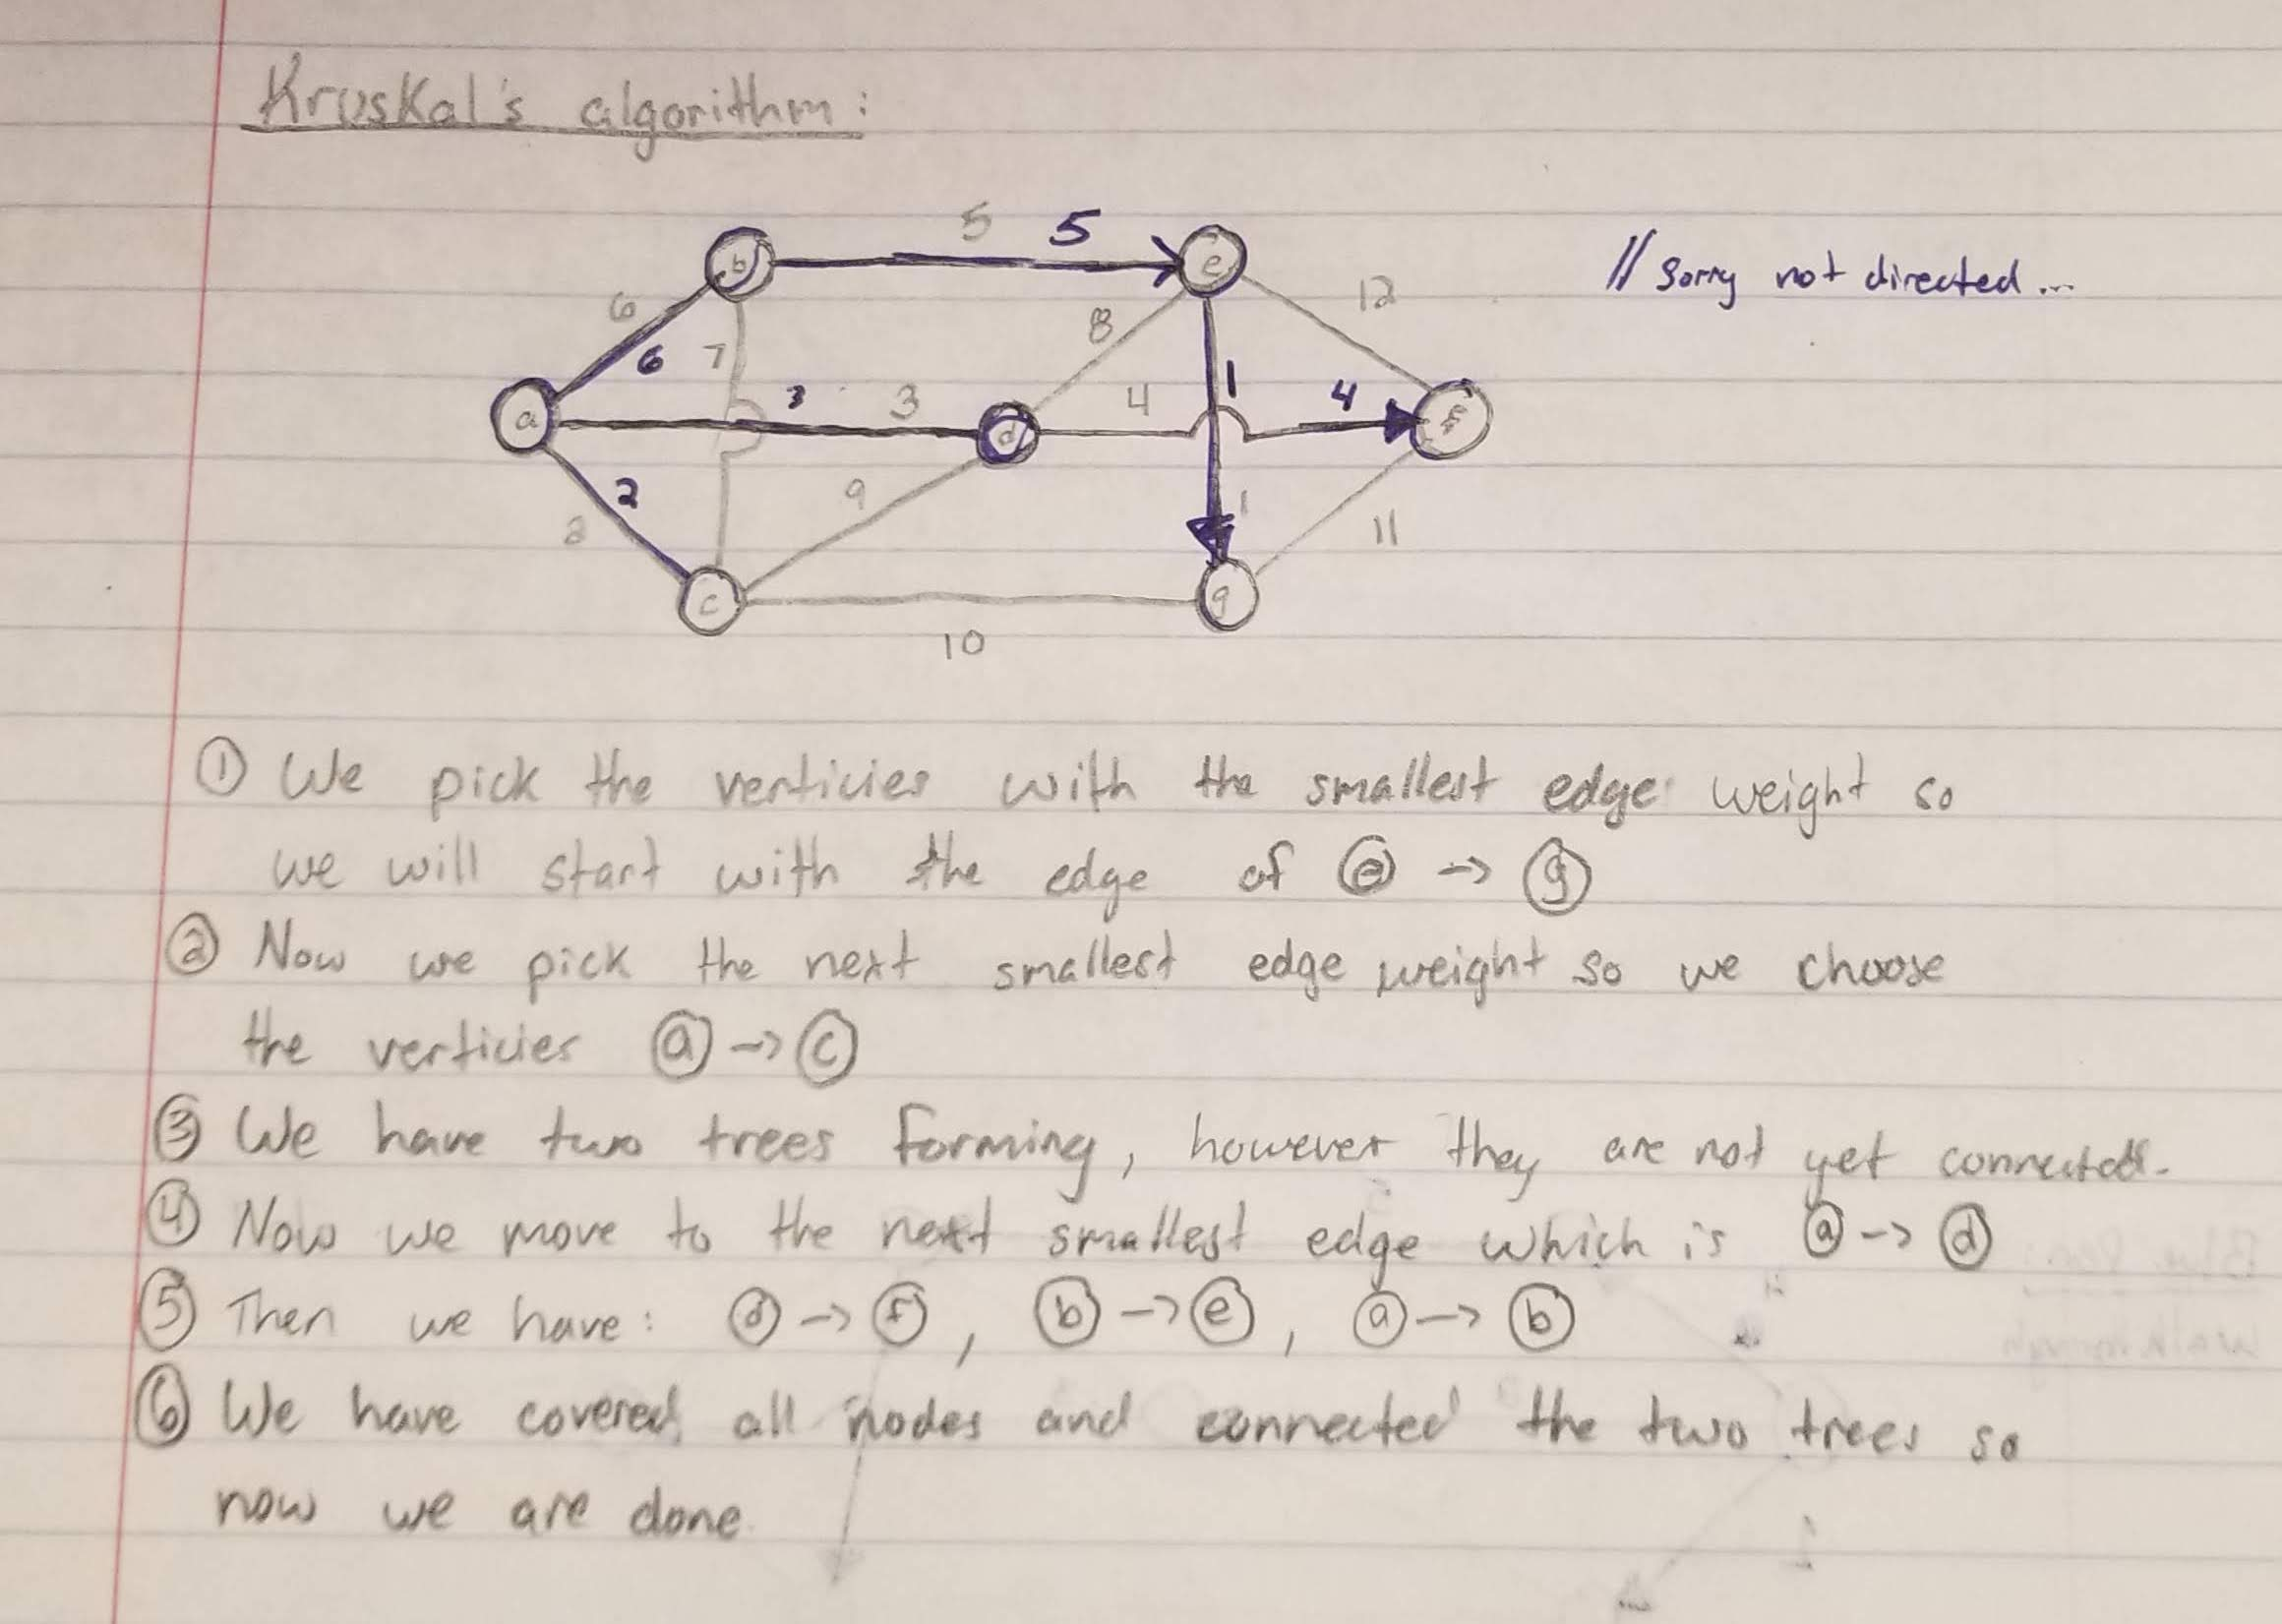
\includegraphics[scale=0.10]{problem3pic5.png}\\
\\
Here is the Boruvka algorithm:\\
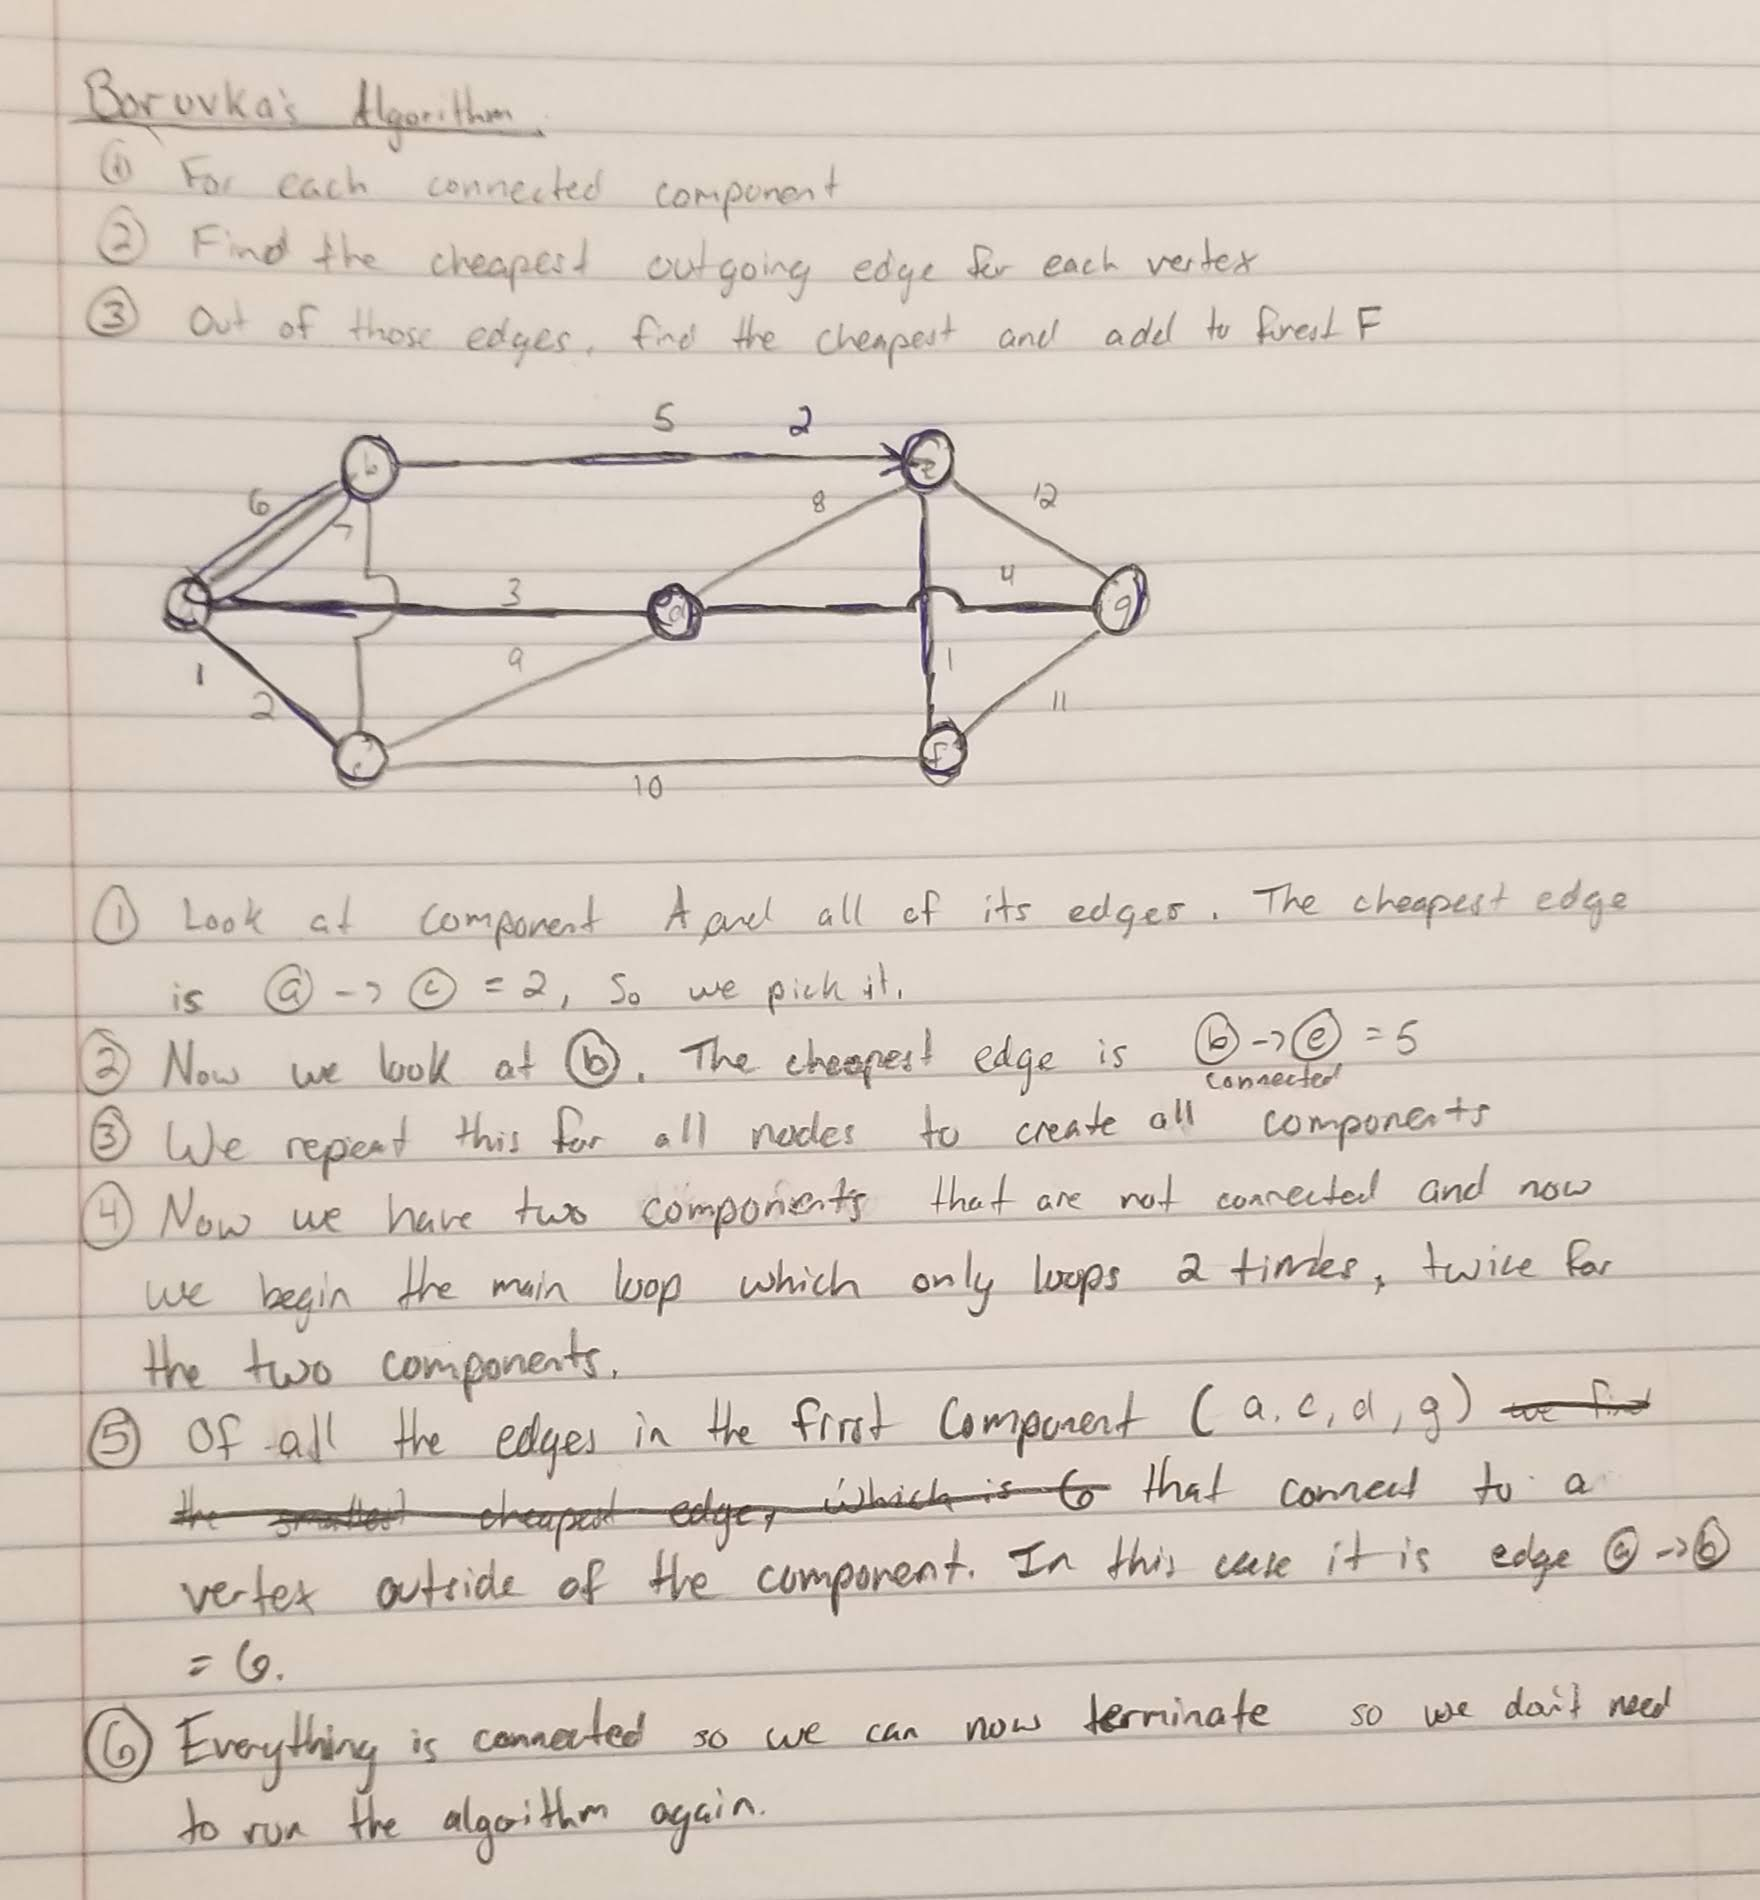
\includegraphics[scale=0.2]{problem3pic6.png}
\\
\\This algorithm creates all of the components on the first iteration and then the second iteration connects the two components together as long as it doesn't break any of the rules.
\\Boruvka is similar to Kruskal's because they both initially create a set of disconnected trees.\\
\\Boruvka looks similar to Prims by how their inner loops operate. Which is so long as we have a disconnected unit we need to keep the loop going. Find the cheapest outgoing edge for each vertex. Then out of those edges, find the cheapest and add to the forest.


	
	

	
\end{enumerate}


\end{document}

